\documentclass{article}

\usepackage{times}
\usepackage[top=1in, bottom=1in, left=1in, right=1in]{geometry}
\usepackage{graphicx}
\usepackage{listings}

\begin{document}

\author{Joshua Ashby\\
        Maurice Ashby\\
        Linux And Sci\\
        \texttt{http://joshashby.com}\\
	\texttt{joshuaashby@joshashby.com}
}
\title{Project: Bouncing Off Bumpers}

  \begin{center}
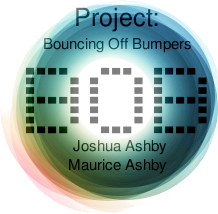
\includegraphics{boblogo}\\
\texttt{http://bob.joshashby.com}\\

In Conjunction with:\\

\includegraphics{linuxandscilogo}\\
\texttt{http://joshashby.com}\\
  \end{center}

\maketitle

\newpage
\tableofcontents
\listoffigures
\renewcommand{\lstlistlistingname}{List of Listings}
\lstlistoflistings

\section{Revisions}\\
March 10th/11th/12th, 2010 - Joshua Ashby\\
Added more to the electronics, Motor controller node part to include the new Quad Low-side V1.5.1 through Revision 3 boards.\\
April 19th, 2010 - Joshua Ashby\\
Added even more to the new sections, cleaning it up, and overall re-writing some parts for better understanding. Rewrote software section also.\\

\newpage

\abstract{Bouncing off Bumpers, or BOB is a competition robot built by Joshua Ashby and his grandfather Maurice Ashby for the April 15th, 2009 Sparkfun Autonomous Vehicle Competition. It measures approximately 3 feet long by 2 feet wide by 2 feet tall; it weights approximately 50 pounds without the battery and electronics.
This paper will go into detail about the many systems involved in the build process of BOB, and provide insight into how many of these systems were designed, and the logic behind them (Please note that this paper is always going to be changing, and the data could easily change the day after the latest pubilishing). BOB has also competed in the 2010 Sparkfun AVC and won the Kill Switch award.}\\

\section{Introduction and Background}
The electronics were designed by me (Joshua Ashby), and built by me along with the aid of my grandfather Maurice Ashby. As of March 10th, 2010 BOB is running on the newly designed and completed Generation 3 electronics. These electronics include the Taco quad-motor Motor controller board with a few minor additions to the board, along with several other monor boards. Over all the design process for the electronics have taken the longest as the motor controllers must be able to meet the demand of 10A per motor, as a result several generation of electronics have gone out the window.\\
The mechanics of the robot, which refers to the frame and body, the steering and related mechanisms, and the propulsion system were designed and built by us over a course of approximately 5 weeks, and has not had any major problems besides the replacement of the front motor.\\
\section{Frame\footnote{Please note, the frame was made to be cheap, and need little maintanince}%
}
\subsection{Shape, Design and Material}
In order to build the frame in both a time and cost effective way, we choose to reuse some old square steel tubing that measures  and has a wall thickness of. My grandfather had just enough laying around his shop to build a frame with. By using steel square tubing, and welding the joints, we were able to build a sturdy frame capable of carrying well over 100LBS over rough terrain.\\
The design of a three wheeled robot came after evaluating the cost of the wheels that would be used; to keep the cost down, only three wheels would be used. Because only three wheels would be used, the frame would have to be built in a fashion that did not promote tilting when the robot turns but still allow a large amount of room to build on top of. To accomplish this, an elongated pentagon design was created. The main drive wheel would be placed at the back of the robot in a triangle shaped portion of the frame, while the middle and front of the body would be a square shape, with two wheels in the front to steer with.\\
\subsection{Steering}
The steering for BOB was modeled after a car style steering system, where two wheels are connected via a rod which is in turn moved left or right to turn the wheels (Figure \ref{steering}).
\begin{figure}[htp]
  \begin{center}
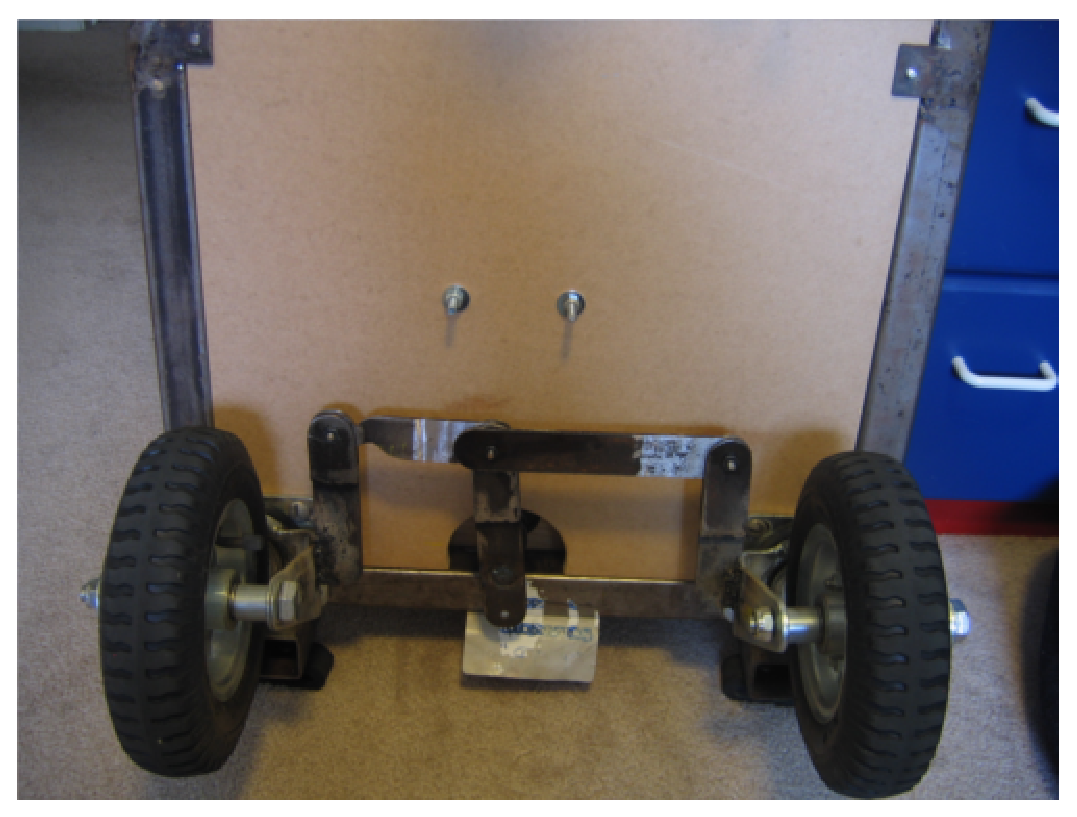
\includegraphics[scale=0.25]{steering}
  \end{center}
  \caption{Example of the steering build used}
\label{steering}
\end{figure}\\
TODO: Fix this description
The build of this was accomplished by using two pre-built wheel casters, and welding on strips of quarter inch thick steel. These strips are approximately 6 inches long, and at the end that is not welded to the caster wheels, there is a hole drilled. Then connecting the two wheels via these strips, is a second pair of steel strips that are hooked up to the steering motor.\\
The steering motor is a 9.6V 10A drill motor that has been mounted with a right angle drive. This allows the motor to lay flat with the robot frame and still be able to turn the steering rod (Figure \ref{steeringmotor}).
\begin{figure}[htp]
  \begin{center}
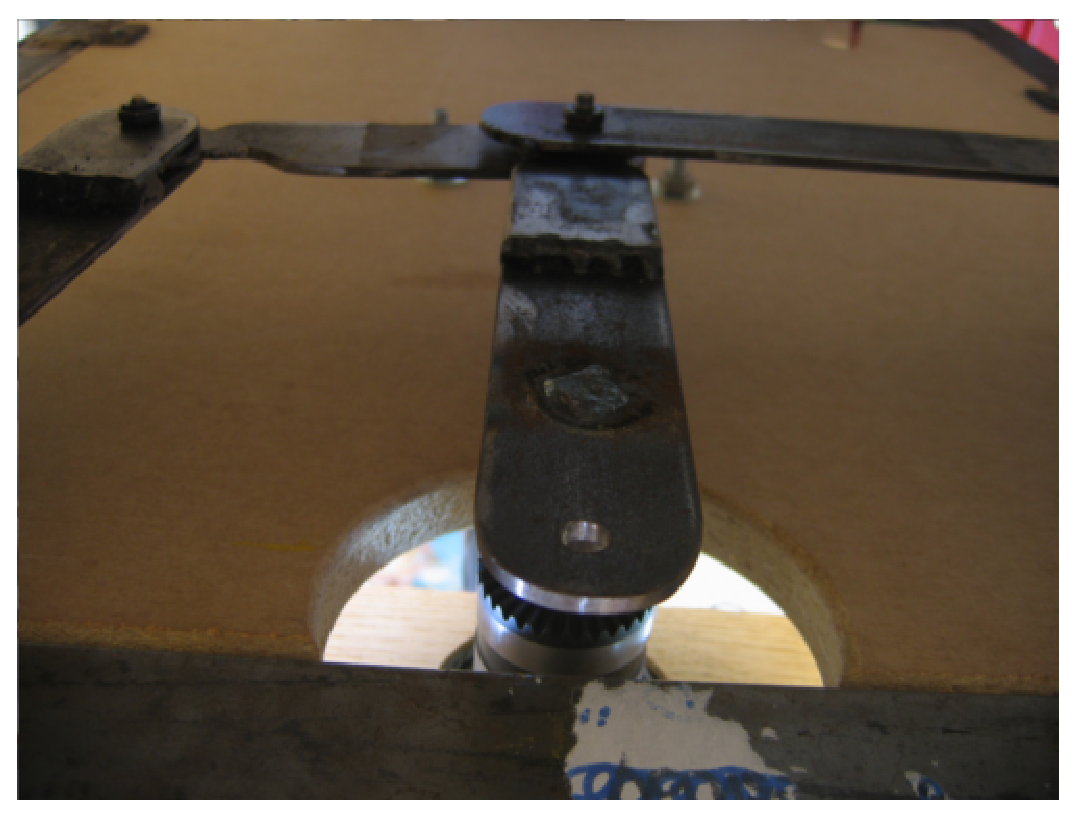
\includegraphics[scale=0.25]{steeringmotor}
  \end{center}
  \caption{Example of the steering motor}
\label{steeringmotor}
\end{figure}\\
One problem that we did not foresee while building the steering, is the ability to drive straight. Because the steering mechanism does not have a method of straighting its self out quickly and effectivly, a new task is introduced to the electronics and programming until further improvments to the steering can be made. This may be accomplished by turning the front motor into an mechanism much like a servo through the use of programming and the ability of the motor controllers, however as of right now, thing has been done to take care of this problem.\\
\subsection{Propulsion}
Transferring power from the drill motor to the back drive wheel was one of the greatest technical difficulties we encountered. We started off by testing the idea of a friction drive. This style of drive has the motor running parallel to the wheel, and the output shaft using friction to turn the wheel. This worked great going downhill, but as soon as the drive had a load to pull, such as on flat ground, or uphill, the drive would start to slip.\\
Our second attempt was based off of a bike, just instead of a chain drive, we decided to do a belt drive as my grandfather had many of the needed parts. The motor was mounted perpendicular to the rotating axis of the wheel, and had a small 1.25 inch radius belt pulley on it. The wheel then had a larger, 2 inch radius, belt pulley on it. The two pulleys were connected via 8 inch diameter cogged belt. The axle for the motor is a milled axle that is supported by a bearing block at one end. The other end is tapered down to allow it to fit in the motor chuck. This also allows the motor to be disconnected from the axle, allowing the robot to be moved around with out power to the motor. (Figure \ref{reardrive}).
\begin{figure}[htp]
  \begin{center}
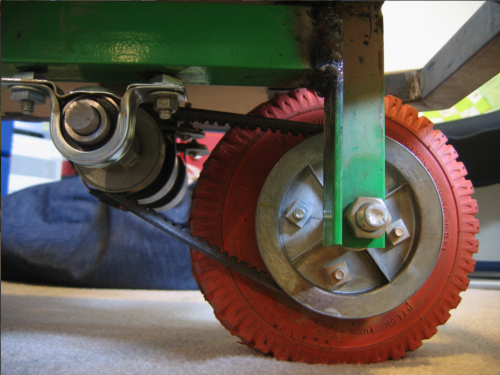
\includegraphics[scale=0.25]{reardrive}
  \end{center}
  \caption{Example of the drive system used}
\label{reardrive}
\end{figure}\\
This drive system worked perfectly both downhill and uphill, and as a result it is the drive system currently used. The motor is the same as the steering motor, a recycled drill motor that is rated at 9.6V and 10A.\\
\section{Electronics}
\subsection{Introduction}
The electronics have always been a troublesome matter for this project and as this is being typed, the electronics still are providing issues, even with new designs.\\
The motors, which each draw ~10A, must have easy to use, and cheap to build motor controllers, along with the ability to easily replace major parts while the robot is not in the Lab or near a soldering iron. This means the motor controllers can not be store bought, as all of the quality controllers that we can find are not only expensive, but also do not have common, easy to find parts. Instead to replace a part, the whole controller must be replaced most the time.\\
Generation 1 electronics consisted of one micro-controller, and one and a half motor controllers. These electronics shorted out at the 2009 Sparkfun AVC competition, and as a result will only be used as both a comparison, and as a resource for what not to do on future generations.\\
\subsection{Motor controller}
As stated above, the use of store bought motor controllers is out of the question for use on BOB. They tend to be expensive, and typically must have the whole unit replaced if something burns out. Because of this, the motor controllers have been hand designed by us.\footnote{Also it's a matter of which is funner to build and use.}\\
The first version, which is the version that was used during the 2009 Sparkfun AVC competition, was designed to be very simple, and yet still provide the power that was needed for the motors. It consisted of a TIP125 PNP transistor driving a pair of paralleled IRF540N n-channel MOSFETs. At the time of their designing and building, we both were very new to MOSFETs and as a result the knowledge of how to hook the MOSFETs up, and the voltage required to drive them was unknown. This caused many problems, such as the MOSFETs not having enough voltage and amperes for them to fully close. This caused them to over heat, and also caused a massive power spike somewhere along the lines that burnt out the MOSFETs and transistor.\\
The new generation 2 motor controllers were designed to avoid these problems, along with begin to merge into a modular system as talked about in section Electronics: Introduction. These new motor controllers werecalled the Motor Nodes, and included two motor controllers, and a micro-controller that talked to the controllers. The micro-controller for generation 2 electronics was an Atmega328p which took care of both the sensors and the motor controllers. The basic design of using the transistors to switch the logic level were used, but with a few improvments such as temperature shut off for the MOSFETs, however it was discovered in late December 2009 that this method of driving the MOSFETs was not atiquate enough, and as a result this method is no longer used. For this reason the Generation 2 electronics have been ditched and new Generation 3 electronics designed and put in place.\\
The new board consists of the main ATmega328P running at 5V with a 16MHz crystal. The I2C headers are broken out\footnote{Which also provide two analog pins for the ultrasounds on BOB}, and the ATmega has 2 LEDs connected to PortD pins 3 and 5, also known as OC2B and OC0B. This allows for PWM debugging of any functions. Next the Atmega is connected to two TC4424CPA chips, one of these chips being on PD1 and PD2, OR1A, OR1B for PWM speed control, and the other chip being on pins PD2, PD4 for simple digital triggering of relays.\\
Along with these new MOSFET drivers, the MOSFET gates have current limiting resistors, and 12V zener diodes to prevent power spikes. The board also has a 10uF and 1000uF capacitor to help smooth out power drops from the motors.\\
This board, which is named Taco is infact a general purpose MOSFET board, but has been desinged in conjunction with BOB for use on him, however the only problem so far has been the traces not being big enough to carry the 10A and 20A from the motors. As a result the board also has several high amperage wires for the MOSFETs and motor outputs.\\
The I2C header is broken out which I2C on the Atmega328p is the analog pins 4 and 5, which means that the board can also be used for analog inputs, such as was used for the ultrasounds on BOB.
\subsection{Power Node}
The Power Node, as of Generation 2 electronics is simply a “dead” Node as one might call it. It has no intelligence, instead it's only function for generation 2 is to regulate and distribute 5V to all the boards. It does this via Molex connectors off of old ATX power supplies from computers. This same board design was used in the Generation 3 electronics also.\\
\section{Software}
\subsection{Libraries - Introduction}
As of January 2010, BOB runs a custom writen library set that takes care of everything from PWM and digital function to analog, ultrasounds, and calibration.
\subsection{Digital Functions}
First up is the digital function library (Page: \pageref{digital}). The digital function library takes care of turning a pin on or off, which seems simple enough. While this task is quite trivial in code, those few extra lines tend to make the code look messy, which I don't like as much.\\
\subsection{Analog Functions}
Unlike the digital code, reading from an analog pin takes some work. First you have to setup the registers, which in my case get me going at a prescaler of 128, interupt driven, and left alinged bits. The left aligned results mean that I don't have to do fancy code and get 10bit results, which I don't need. instead I can simply read the ADCH register and get an 8 bit result. The next step is to read the results, or change the pin that I am reading from, both which take more code. As a result of all this, placing the analog functions inside of a nice, clean library makes sense (Page: \pageref{analog}).\\
\subsection{PWM Functions}
Like the analog functions, the PWM functions that I needed were large, and very messy pieces of code. They consisted of several functions that setup the registers for the three PWM timers, and then several more to add in functions like ramp up and down functionability. (Page: \pageref{pwm}).\\
\subsection{Robotics Functions}
The robotics library takes care of most of the things that BOB needs to run. It houses the turn functions, and the filter that takes care of the  ultrasound data. This filter is a custom rolling average with a few additions which smooth the data points out really well as the analog outputs on the ultrasounds are a little jumpy (Page: \pageref{robot}).\\
\subsection{Boot Functions}
Finally the boot library takes care of setting everything up as the robot first starts, basically it's an implementation of a low level bios for BOB (Page: \pageref{boot}).\\
\newpage
\section{About the builders}
\subsection{Joshua Ashby}
\subsection{Maurice Ashby}

\newpage
\section{Appendix}
All code and schematics are released under the Creative Commons Attribution-Noncommercial 3.0 United States License.\\
The code can be found online at github: http://github.com/JoshAshby/Robotbob/tree/experimental\\
\subsection{Code}
\lstset{language=C}
\lstset{numbers=left, numberstyle=\small, stepnumber=1, numbersep=5pt}
\begin{lstlisting}[caption={The digital function library.},label=digital,frame=tbl]

//-------------------------------------------
/*
DIGITAL.h
2010 - Josh Ashby
joshuaashby@joshashby.com
http://joshashby.com
http://github.com/JoshAshby
freenode/#linuxandsci - JoshAshby
*/
//-------------------------------------------
#include "adc.h"
#include "pwm.h"
#include "digital.h"
#include "boot.h"
#include "global.h"
#include "robotfunc.h"
//add the ability for it to auto detect which port based on what pin number you give
void portB_out(int pin, int value)
{
    if (value == 0)
    {
        PORTB &= ~(1<<pin);
    }
    else
    {
        PORTB |= (1<<pin);
    }
}
void portD_out(int pin, int value)
{
    if (value == 0)
    {
        PORTD &= ~(1<<pin);
    }
    else
    {
        PORTD |= (1<<pin);
    }
}
void out(char port, int pin, int value){
    switch (port) {
        case 'D':
            if(value == 1){
                PORTD |= (1<<pin);
            }
            else {
                PORTD &= ~(1<<pin);
            }
            break;
        case 'B':
            if(value == 1){
                PORTB |= (1<<pin);
            }
            else {
                PORTB &= ~(1<<pin);
            }
            break;
    }
}


\end{lstlisting}

\begin{lstlisting}[caption={The analog function library.},label=analog,frame=tbl]
//-------------------------------------------
/*
ADC.c
2010 - Josh Ashby
joshuaashby@joshashby.com
http://joshashby.com
http://github.com/JoshAshby
freenode/#linuxandsci - JoshAshby
*/
//-------------------------------------------
#include "adc.h"
#include "pwm.h"
#include "digital.h"
#include "boot.h"
#include "global.h"
#include "robotfunc.h"
ISR(ADC_vect)
{
}
void adc_start(void)
{
    ADCSRA |= (1 << ADPS2)
            | (1 << ADPS1)
            | (1 << ADPS0); // Set ADC prescaler to 128 - 125KHz sample rate @ 16MHz
    ADMUX |= (1 << REFS0); // Set ADC reference to AVCC
    ADMUX |= (1 << ADLAR); // Left adjust ADC result to allow easy 8 bit reading
    ADCSRA |= (1 << ADATE);
    ADCSRA |= (1 << ADEN);  // Enable ADC
    ADCSRA |= (1 << ADIE);  // Enable ADC Interrupt
    sei();
    ADCSRA |= (1 << ADSC);  // Start A2D Conversions
}
void adc_stop(){
    //stop the ADC
    ADCSRA &= ~(1 << ADSC);
}
void adc_change(int chan){
    //stop the ADC
    ADCSRA &= ~(1 << ADSC);
    //and now change the ADMUX bits to fit which channal
    //you want to use, this should probably be replaced by a switch soon
    switch (chan) {
        case 0:
            ADMUX &= ~(1 << MUX0)
                  &  ~(1 << MUX1)
                  &  ~(1 << MUX2)
                  &  ~(1 << MUX3);
            break;
        case 1:
            ADMUX |=  (1 << MUX0);
            ADMUX &= ~(1 << MUX1)
                  &  ~(1 << MUX2)
                  &  ~(1 << MUX3);
            break;
        case 2:
            ADMUX &= ~(1 << MUX0);
            ADMUX |=  (1 << MUX1);
            ADMUX &= ~(1 << MUX2)
                  &  ~(1 << MUX3);
            break;
        case 3:
            ADMUX |=  (1 << MUX0)
                  |   (1 << MUX1);
            ADMUX &= ~(1 << MUX2)
                  &  ~(1 << MUX3);
            break;
        case 4:
            ADMUX &= ~(1 << MUX0)
                  &  ~(1 << MUX1);
            ADMUX |=  (1 << MUX2);
            ADMUX &= ~(1 << MUX3);
            break;
        case 5:
            ADMUX |=  (1 << MUX0);
            ADMUX &= ~(1 << MUX1);
            ADMUX |=  (1 << MUX2);
            ADMUX &= ~(1 << MUX3);
            break;
        case 6:
            ADMUX &= ~(1 << MUX0);
            ADMUX |=  (1 << MUX1)
                  |   (1 << MUX2);
            ADMUX &= ~(1 << MUX3);
            break;
        case 7:
            ADMUX |=  (1 << MUX0)
                  |   (1 << MUX1)
                  |   (1 << MUX2);
            ADMUX &= ~(1 << MUX3);
            break;
        case 8:
            ADMUX &= ~(1 << MUX0)
                  &  ~(1 << MUX1)
                  &  ~(1 << MUX2);
            ADMUX |=  (1 << MUX3);
            break;
    }
    ADCSRA |= (1 << ADSC);
}

\end{lstlisting}


\begin{lstlisting}[caption={The PWM function library.},label=pwm,frame=tbl]
//-------------------------------------------
/*
PWM.c
2010 - Josh Ashby
joshuaashby@joshashby.com
http://joshashby.com
http://github.com/JoshAshby
freenode/#linuxandsci - JoshAshby
*/
//-------------------------------------------
#include "adc.h"
#include "pwm.h"
#include "digital.h"
#include "boot.h"
#include "global.h"
#include "robotfunc.h"
void pwm_setup_all(void){
    TCCR0B |= (1<<CS00)
            | (1<<CS01);
    TCCR0A |= (1<<WGM00);

    DDRD |= (1<<5);
    DDRD |= (1<<6);

    pwm_speed0A = 0;
    pwm_value0A = 0;
    pwm_value_old0A = 0;

    pwm_speed0B = 0;
    pwm_value0B = 0;
    pwm_value_old0B = 0;

    TCCR1B |= (1<<CS11)
            | (1<<CS10);
    TCCR1A |= (1<<WGM10);

    DDRB |= (1<<1);
    DDRB |= (1<<2);

    pwm_speed1A = 0;
    pwm_value1A = 0;
    pwm_value_old1A = 0;

    pwm_speed1B = 0;
    pwm_value1B = 0;
    pwm_value_old1B = 0;

    TCCR2B |= (1<<CS22);
    TCCR2A |= (1<<WGM20);

    DDRD |= (1<<3);
    DDRB |= (1<<3);

    pwm_speed2A = 0;
    pwm_value2A = 0;
    pwm_value_old2A = 0;

    pwm_speed2B = 0;
    pwm_value2B = 0;
    pwm_value_old2B = 0;
}
void pwm_setup0(void)
{
    TCCR0B |= (1<<CS00)
            | (1<<CS01);
    TCCR0A |= (1<<WGM00);

    DDRD |= (1<<5);
    DDRD |= (1<<6);

    pwm_speed0A = 0;
    pwm_value0A = 0;
    pwm_value_old0A = 0;

    pwm_speed0B = 0;
    pwm_value0B = 0;
    pwm_value_old0B = 0;
}
void pwm0A(unsigned int value)//set the duty cycle on the PWM
{
    TCCR0A |= (1<<COM0A1);
    OCR0A = value;
}
void pwm0B(unsigned int value)//set the duty cycle on the PWM
{
    TCCR0A |= (1<<COM0B1);
    OCR0B = value;
}
//calling any of these wll stop the processor for a short amonnt of time due to the delay
void pwm_ramp0A(unsigned int value, unsigned int speed)
{
    if (value == 0) {//safe gaurd to prevent i from over flowing
        pwm0A(0);
    }
    else {
    if (value > pwm_value_old1A){//determine if it should ramp up or down
        TCCR0A |= (1<<COM0A1);
        unsigned int i = pwm_value_old0A;
        while (i<=value) {//ramp up
            OCR0A=i;
            i++;
            _delay_ms(speed);
        }
        pwm_value_old0A = value;//store the old pwm for autoramping
    } else {
        TCCR0A |= (1<<COM0A1);
        unsigned int i = pwm_value_old0A;
        while (i>=value) {//ramp down
            OCR0A=i;
            i--;
            _delay_ms(speed);
        }
    }
        pwm_value_old0A = value;//store the old pwm for autoramping
    }
}
void pwm_rampUp0A(unsigned int value, unsigned int speed)
{
    TCCR0A |= (1<<COM0A1);
    unsigned int i = pwm_value_old0A;
    while (i<=value) {//ramp up
        OCR0A=i;
        i++;
        _delay_ms(speed);
    }
    pwm_value_old0A = value;//store the old pwm for autoramping
}
void pwm_rampDown0A(unsigned int value, unsigned int speed)
{
    if (value == 0) {//safe gaurd to prevent i from over flowing
        pwm0A(0);
    }
    else {
    TCCR0A |= (1<<COM0A1);
    unsigned int i = pwm_value_old0A;
    while (i>=value) {//ramp down
        OCR0A=i;
        i--;
        _delay_ms(speed);
    }
    }
    pwm_value_old0A = value;//store the old pwm for autoramping
}


void pwm_ramp0B(unsigned int value, unsigned int speed)
{
    if (value == 0) {//safe gaurd to prevent i from over flowing
        pwm0B(0);
    }
    if (value > pwm_value_old0B){//determine if it should ramp up or down
        TCCR0A |= (1<<COM0B1);
        unsigned int i = pwm_value_old0B;
        while (i<=value) {//ramp up
            OCR0B=i;
            i++;
            _delay_ms(speed);
        }
        pwm_value_old0B = value;//store the old pwm for autoramping
    } else {
        TCCR0A |= (1<<COM0B1);
        unsigned int i = pwm_value_old0B;
        while (i>=value) {//ramp down
            OCR0B=i;
            i--;
            _delay_ms(speed);
        }
        pwm_value_old0B = value;//store the old pwm for autoramping
    }
}
void pwm_rampUp0B(unsigned int value, unsigned int speed)
{
    TCCR0A |= (1<<COM0B1);
    unsigned int i = pwm_value_old0B;
    while (i<=value) {//ramp up
        OCR0B=i;
        i++;
        _delay_ms(speed);
    }
    pwm_value_old0B = value;//store the old pwm for autoramping
}
void pwm_rampDown0B(unsigned int value, unsigned int speed)
{
    if (value == 0) {//safe gaurd to prevent i from over flowing
        pwm0B(0);
    }
    TCCR0A |= (1<<COM0B1);
    unsigned int i = pwm_value_old0B;
    while (i>=value) {//ramp down
        OCR1B=i;
        i--;
        _delay_ms(speed);
    }
    pwm_value_old0B = value;//store the old pwm for autoramping
}

//-------------------------------------------
void pwm_setup1(void)
{
    TCCR1B |= (1<<CS11)
            | (1<<CS10);
    TCCR1A |= (1<<WGM10);

    DDRB |= (1<<1);
    DDRB |= (1<<2);

    pwm_speed1A = 0;
    pwm_value1A = 0;
    pwm_value_old1A = 0;

    pwm_speed1B = 0;
    pwm_value1B = 0;
    pwm_value_old1B = 0;
}
void pwm1A(int value)//set the duty cycle on the PWM
{
    TCCR1A |= (1<<COM1A1);
    OCR1A = value;
}
void pwm1B(unsigned int value)//set the duty cycle on the PWM
{
    TCCR1A |= (1<<COM1B1);
    OCR1B = value;
}
//calling any of these wll stop the processor for a short amonnt of time due to the delay
void pwm_ramp1A(int value, int speed)
{
    if (value == 0) {//safe gaurd to prevent i from over flowing
        pwm1A(0);
    }
    else {
    if (value > pwm_value_old1A){//determine if it should ramp up or down
        TCCR1A |= (1<<COM1A1);
        unsigned int i = pwm_value_old1A;
        while (i<=value) {//ramp up
            OCR1A=i;
            i++;
            _delay_ms(speed);
        }
        pwm_value_old1A = value;//store the old pwm for autoramping
    } else {
        TCCR1A |= (1<<COM1A1);
        unsigned int i = pwm_value_old1A;
        while (i>=value) {//ramp down
            OCR1A=i;
            i--;
            _delay_ms(speed);
        }
    }
        pwm_value_old1A = value;//store the old pwm for autoramping
    }
}
void pwm_rampUp1A(unsigned int value, unsigned int speed)
{
    TCCR1A |= (1<<COM1A1);
    unsigned int i = pwm_value_old1A;
    while (i<=value) {//ramp up
        OCR1A=i;
        i++;
        _delay_ms(speed);
    }
    pwm_value_old1A = value;//store the old pwm for autoramping
}
void pwm_rampDown1A(unsigned int value, unsigned int speed)
{
    if (value == 0) {//safe gaurd to prevent i from over flowing
        pwm1A(0);
    }
    else {
    TCCR1A |= (1<<COM1A1);
    unsigned int i = pwm_value_old1A;
    while (i>=value) {//ramp down
        OCR1A=i;
        i--;
        _delay_ms(speed);
    }
    }
    pwm_value_old1A = value;//store the old pwm for autoramping
}


void pwm_ramp1B(unsigned int value, unsigned int speed)
{
    if (value == 0) {//safe gaurd to prevent i from over flowing
        pwm1B(0);
    }
    if (value > pwm_value_old1B){//determine if it should ramp up or down
        TCCR1A |= (1<<COM1B1);
        unsigned int i = pwm_value_old1B;
        while (i<=value) {//ramp up
            OCR1B=i;
            i++;
            _delay_ms(speed);
        }
        pwm_value_old1B = value;//store the old pwm for autoramping
    } else {
        TCCR1A |= (1<<COM1B1);
        unsigned int i = pwm_value_old1B;
        while (i>=value) {//ramp down
            OCR1B=i;
            i--;
            _delay_ms(speed);
        }
        pwm_value_old1B = value;//store the old pwm for autoramping
    }
}
void pwm_rampUp1B(unsigned int value, unsigned int speed)
{
    TCCR1A |= (1<<COM1B1);
    unsigned int i = pwm_value_old1B;
    while (i<=value) {//ramp up
        OCR1B=i;
        i++;
        _delay_ms(speed);
    }
    pwm_value_old1B = value;//store the old pwm for autoramping
}
void pwm_rampDown1B(unsigned int value, unsigned int speed)
{
    if (value == 0) {//safe gaurd to prevent i from over flowing
        pwm1B(0);
    }
    TCCR1A |= (1<<COM1B1);
    unsigned int i = pwm_value_old1B;
    while (i>=value) {//ramp down
        OCR1B=i;
        i--;
        _delay_ms(speed);
    }
    pwm_value_old1B = value;//store the old pwm for autoramping
}
//--------------------------------------------
void pwm_setup2(void)
{
    TCCR2B |= (1<<CS22);
    TCCR2A |= (1<<WGM20);

    DDRD |= (1<<3);
    DDRB |= (1<<3);

    pwm_speed2A = 0;
    pwm_value2A = 0;
    pwm_value_old2A = 0;

    pwm_speed2B = 0;
    pwm_value2B = 0;
    pwm_value_old2B = 0;
}
void pwm2A(unsigned int value)//set the duty cycle on the PWM
{
    TCCR2A |= (1<<COM2A1);
    OCR2A = value;
}
void pwm2B(unsigned int value)//set the duty cycle on the PWM
{
    TCCR2A |= (1<<COM2B1);
    OCR2B = value;
}
//calling any of these wll stop the processor for a short amonnt of time due to the delay
void pwm_ramp2A(unsigned int value, unsigned int speed)
{
    if (value == 0) {//safe gaurd to prevent i from over flowing
        pwm2A(0);
    }
    else {
    if (value > pwm_value_old2A){//determine if it should ramp up or down
        TCCR2A |= (1<<COM2A1);
        unsigned int i = pwm_value_old2A;
        while (i<=value) {//ramp up
            OCR2A=i;
            i++;
            _delay_ms(speed);
        }
        pwm_value_old2A = value;//store the old pwm for autoramping
    } else {
        TCCR2A |= (1<<COM2A1);
        unsigned int i = pwm_value_old2A;
        while (i>=value) {//ramp down
            OCR2A=i;
            i--;
            _delay_ms(speed);
        }
    }
        pwm_value_old2A = value;//store the old pwm for autoramping
    }
}
void pwm_rampUp2A(unsigned int value, unsigned int speed)
{
    TCCR2A |= (1<<COM2A1);
    unsigned int i = pwm_value_old2A;
    while (i<=value) {//ramp up
        OCR2A=i;
        i++;
        _delay_ms(speed);
    }
    pwm_value_old2A = value;//store the old pwm for autoramping
}
void pwm_rampDown2A(unsigned int value, unsigned int speed)
{
    if (value == 0) {//safe gaurd to prevent i from over flowing
        pwm2A(0);
    }
    else {
    TCCR2A |= (1<<COM2A1);
    unsigned int i = pwm_value_old2A;
    while (i>=value) {//ramp down
        OCR2A=i;
        i--;
        _delay_ms(speed);
    }
    }
    pwm_value_old2A = value;//store the old pwm for autoramping
}


void pwm_ramp2B(unsigned int value, unsigned int speed)
{
    if (value == 0) {//safe gaurd to prevent i from over flowing
        pwm2B(0);
    }
    if (value > pwm_value_old2B){//determine if it should ramp up or down
        TCCR2A |= (1<<COM2B1);
        unsigned int i = pwm_value_old2B;
        while (i<=value) {//ramp up
            OCR2B=i;
            i++;
            _delay_ms(speed);
        }
        pwm_value_old2B = value;//store the old pwm for autoramping
    } else {
        TCCR2A |= (1<<COM2B1);
        unsigned int i = pwm_value_old2B;
        while (i>=value) {//ramp down
            OCR2B=i;
            i--;
            _delay_ms(speed);
        }
        pwm_value_old2B = value;//store the old pwm for autoramping
    }
}
void pwm_rampUp2B(unsigned int value, unsigned int speed)
{
    TCCR2A |= (1<<COM2B1);
    unsigned int i = pwm_value_old2B;
    while (i<=value) {//ramp up
        OCR2B=i;
        i++;
        _delay_ms(speed);
    }
    pwm_value_old2B = value;//store the old pwm for autoramping
}
void pwm_rampDown2B(unsigned int value, unsigned int speed)
{
    if (value == 0) {//safe gaurd to prevent i from over flowing
        pwm2B(0);
    }
    TCCR2A |= (1<<COM2B1);
    unsigned int i = pwm_value_old2B;
    while (i>=value) {//ramp down
        OCR2B=i;
        i--;
        _delay_ms(speed);
    }
    pwm_value_old2B = value;//store the old pwm for autoramping
}

\end{lstlisting}

\begin{lstlisting}[caption={The robotics function library.},label=robot,frame=tbl]
#include "adc.h"
#include "pwm.h"
#include "digital.h"
#include "boot.h"
#include "global.h"
#include "robotfunc.h"
#include <util/delay.h>
//-------------------------------------------
/*
robotfunc.c
2010 - Josh Ashby
joshuaashby@joshashby.com
http://joshashby.com
http://github.com/JoshAshby
freenode/#linuxandsci - JoshAshby
*/
//-------------------------------------------

void turn_left(void){
    out('D', 4, 1);
    _delay_ms(5);
    pwm1B(255);
    _delay_ms(200);
    pwm1B(0);
    out('D', 4, 0);
}
void turn_right(void){
    pwm1B(255);
    _delay_ms(150);
    pwm1B(0);
}
void stop(void){
    pwm0A(0);
    pwm0B(0);
    pwm1A(0);
    pwm1B(0);
    pwm2A(0);
    pwm2B(0);
    out('D', 2, 1);
    error(1);
    out('D', 4, 0);
    out('D', 5, 0);
}
void calibrate(void){
    adc_change(5);
    _delay_ms(20);
    adc = ADCH;
    for (j = 0; j <= 20; j++){
        if (ADCH > average + 100)
        {
            adc = (ADCH/2) + (average/2);
        }
        if (ADCH < average - 100){
            adc = (ADCH/2) + (average/2);
        }
        rollAverage[j] = adc;
    }
    for (j = 0; j <= 20; j++){
        average += rollAverage[j];
    }
    average = average/18;
    base = average;
    for (j = 0; j <= 20; j++){
        rollAverage[j] = 0;
    }
}
int ultrasound_filter(int pin){
    /*simple filter that works quite well, it simply
    smooths out the ADC data from the ultrasounds
    if the ADCH data is out of range, it will divide
    it by two, and then add the average divided by two*/
    adc_change(pin);
    _delay_ms(20);
    adc = ADCH;
    for (j = 0; j <= 30; j++){
        if (ADCH > average + 100)
        {
            adc = (ADCH/2) + (average/2);
        }
        if (ADCH < average - 100){
            adc = (ADCH/2) + (average/2);
        }
        rollAverage[j] = adc;
    }
    for (j = 0; j <= 30; j++){
        average += rollAverage[j];
    }
    average = average/30;
    return average;
}
void ultrasound_test(void){
    if (ultrasound_filter(4) >= base) {
        out('D', 2, 0);
        pwm2B(ultrasound_filter(5));
    } else {
        out('D', 2, 1);
        pwm2B(ultrasound_filter(4));
    }
}
void test_turn(void){
    out('B', 2, 1);
    _delay_ms(200);
    out('B', 2, 0);
    _delay_ms(200);
    out('D', 4, 1);
    _delay_ms(500);
    out('B', 2, 1);
    _delay_ms(200);
    out('B', 2, 0);
    _delay_ms(500);
    out('D', 4, 0);
    _delay_ms(500);
}
void test_motor(void){
    pwm_ramp1A(255, 10);
    _delay_ms(2000);
    pwm_ramp1A(1, 0);
    pwm1A(0);
    _delay_ms(500);
    out('D', 5, 1);
    _delay_ms(500);
    pwm_ramp1A(255, 10);
    _delay_ms(2000);
    pwm_ramp1A(1, 0);
    pwm1A(0);
    _delay_ms(500);
    out('D', 5, 0);
}

\end{lstlisting}

\begin{lstlisting}[caption={The boot function library.},label=boot,frame=tbl]
#include "adc.h"
#include "pwm.h"
#include "digital.h"
#include "boot.h"
#include "global.h"
#include "robotfunc.h"
#include <util/delay.h>

//-------------------------------------------
/*
Boot.c
2010 - Josh Ashby
joshuaashby@joshashby.com
http://joshashby.com
http://github.com/JoshAshby
freenode/#linuxandsci - JoshAshby
*/
//-------------------------------------------
//add a basica bios that will take, start the ADC
//calibrate the sensors to what value they should try to stay at
//also go through and make sure everything is working from what it
//can tell if there is an error then it will blink the status led
void all_good(){//turn the status led on
    out('D', 3, 1);
}
void oh_crap(){//status led off
    out('D', 3, 0);
}
void error(int type){//blink the status led if there is an error
    switch (type) {
        case 0:
            out('D', 3, 1);
            _delay_ms(500);
            out('D', 3, 0);
            _delay_ms(500);
            break;
        case 1:
            pwm_ramp2B(255, 10);
            pwm_ramp2B(1, 10);
            break;
        case 2:
            pwm_ramp2B(255, 50);
            pwm_ramp2B(0, 10);
            break;
    }
}
void bios(){
    DDRD |= (1<<2);//LED power
    DDRD |= (1<<3);//LED Status
    DDRD |= (1<<4);//relay back
    DDRD |= (1<<5);//relay front
    out('D', 2, 1);//CPU power LED
    pwm_setup_all();
    adc_start();//because we're using interrupts ADCH will auto update
    calibrate();
    all_good();
}

\end{lstlisting}

\end{document}
